\documentclass{standalone}

\usepackage{tikz,pgfplots}
\usepackage{xcolor}
\pgfplotsset{compat=newest} % change newest to current version

\newcommand{\N}{5}

% the Barbie colours https://coolors.co/66b7d5-846566-6e1e2f-aac6d6-bd678b
\definecolor{below}{RGB}{102,183,213} % https://www.wolframalpha.com/input?i=convert+%2366B7D5+to+RGB
\definecolor{neutral}{RGB}{110,30,47} % https://www.wolframalpha.com/input?i=convert+%236E1E2F+to+RGB
\definecolor{above}{RGB}{189,103,139} % https://www.wolframalpha.com/input?i=convert+%23BD678B+to+RGB

\begin{document}
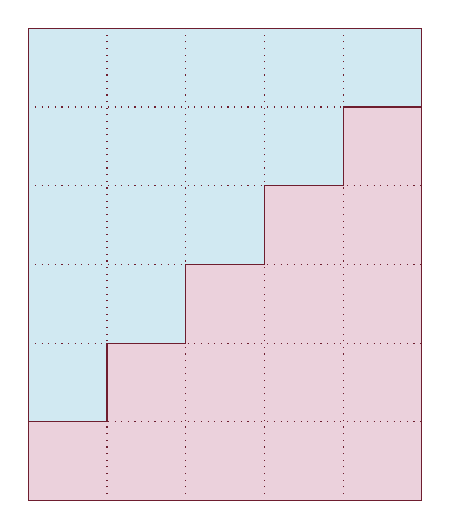
\begin{tikzpicture}
  \foreach \x in {1,...,\N} {
    \fill[fill=above!30] ({\x-1},0) rectangle ++(1,\x);
  }

  \foreach \x in {1,...,\N} {
    \fill[fill=below!30] ({\x-1},\N+1) rectangle ++(1,{-\N+\x-1});
  }

  \draw[dotted, neutral] (0,0) grid[step=1] (\N, \N+1);
  \draw[neutral] (0,0) 
    -- ++(0,1) -- ++(1,0)
    -- ++(0,1) -- ++(1,0)
    -- ++(0,1) -- ++(1,0)
    -- ++(0,1) -- ++(1,0)
    -- ++(0,1) -- ++(1,0)
    -- ++(0,1);
  \draw[neutral] (0,0) -- (\N,0) -- (\N, \N+1) -- (0, \N+1) -- (0,0);
\end{tikzpicture}
\end{document}

